\documentclass{standalone}
\usepackage{tikz}
\usetikzlibrary{patterns, positioning}


\begin{document}
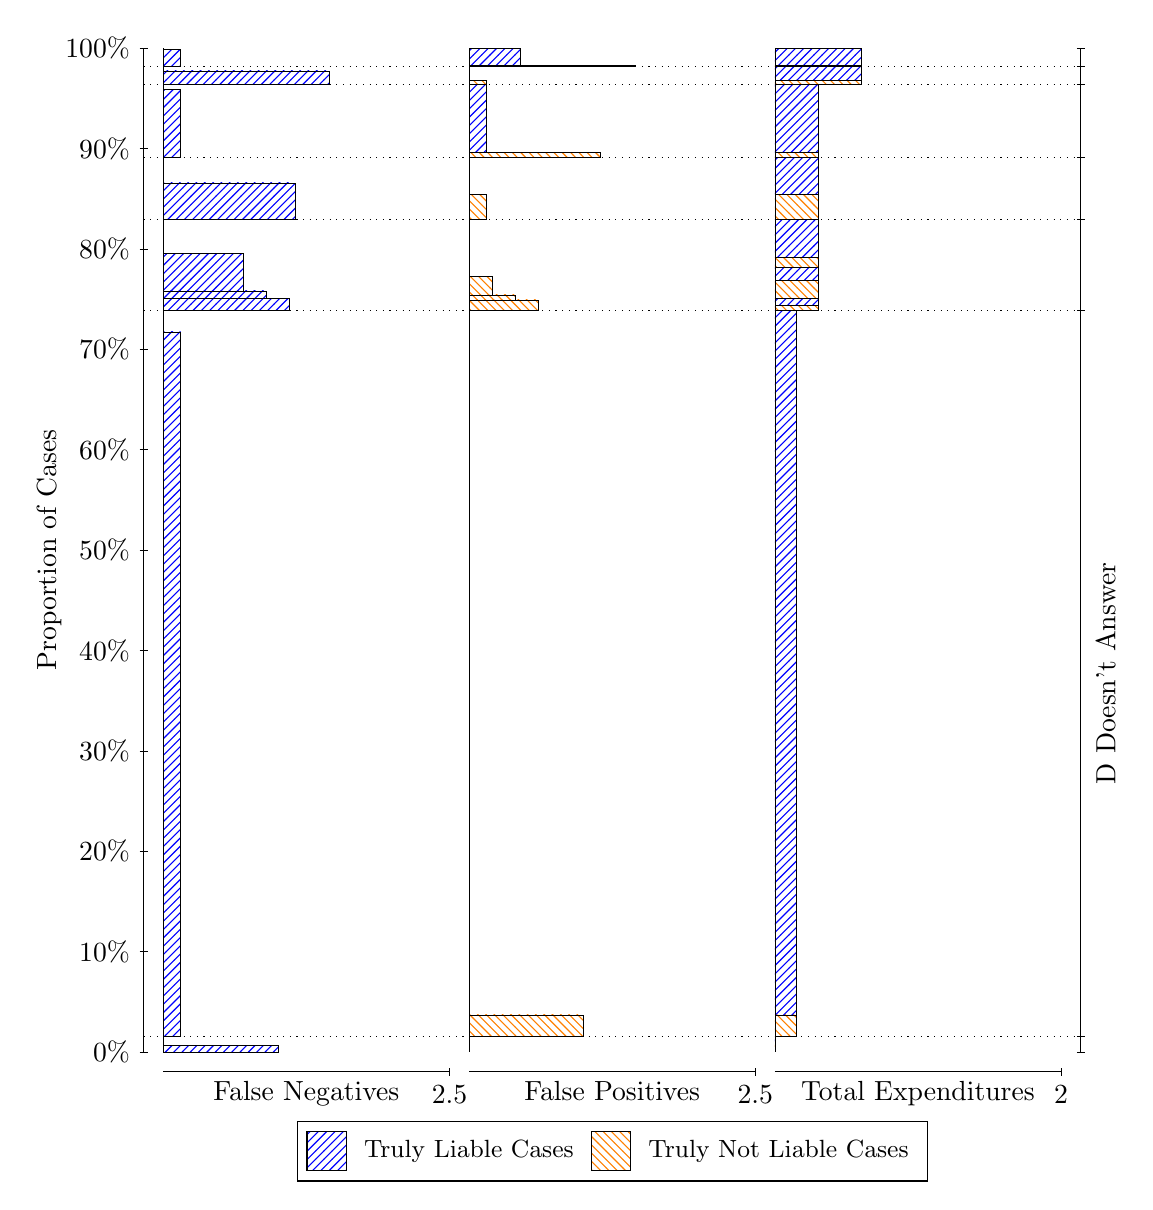
\begin{tikzpicture}
\draw[black, very thin] (1.5,1.75) -- (1.5,14.5);
\node[rotate=90, text=black, anchor=center] at (0.3, 8.125) {Proportion of Cases};
\draw[black, very thin] (1.45,1.75) -- (1.55,1.75);
\node[text=black, anchor=east] at (1.45, 1.75) {0\%};
\draw[black, very thin] (1.45,3.025) -- (1.55,3.025);
\node[text=black, anchor=east] at (1.45, 3.025) {10\%};
\draw[black, very thin] (1.45,4.3) -- (1.55,4.3);
\node[text=black, anchor=east] at (1.45, 4.3) {20\%};
\draw[black, very thin] (1.45,5.575) -- (1.55,5.575);
\node[text=black, anchor=east] at (1.45, 5.575) {30\%};
\draw[black, very thin] (1.45,6.85) -- (1.55,6.85);
\node[text=black, anchor=east] at (1.45, 6.85) {40\%};
\draw[black, very thin] (1.45,8.125) -- (1.55,8.125);
\node[text=black, anchor=east] at (1.45, 8.125) {50\%};
\draw[black, very thin] (1.45,9.4) -- (1.55,9.4);
\node[text=black, anchor=east] at (1.45, 9.4) {60\%};
\draw[black, very thin] (1.45,10.675) -- (1.55,10.675);
\node[text=black, anchor=east] at (1.45, 10.675) {70\%};
\draw[black, very thin] (1.45,11.95) -- (1.55,11.95);
\node[text=black, anchor=east] at (1.45, 11.95) {80\%};
\draw[black, very thin] (1.45,13.225) -- (1.55,13.225);
\node[text=black, anchor=east] at (1.45, 13.225) {90\%};
\draw[black, very thin] (1.45,14.5) -- (1.55,14.5);
\node[text=black, anchor=east] at (1.45, 14.5) {100\%};

\draw[black, very thin] (13.4,1.75) -- (13.4,14.5);
\draw[black, very thin] (13.35,1.75) -- (13.45,1.75);
\node[anchor=west] at (13.35, 1.75) {};
\draw[black, very thin] (13.35,1.9488) -- (13.45,1.9488);
\node[anchor=west] at (13.35, 1.9488) {};
\draw[black, very thin] (13.35,11.166) -- (13.45,11.166);
\node[anchor=west] at (13.35, 11.166) {};
\draw[black, very thin] (13.35,12.32) -- (13.45,12.32);
\node[anchor=west] at (13.35, 12.32) {};
\draw[black, very thin] (13.35,13.109) -- (13.45,13.109);
\node[anchor=west] at (13.35, 13.109) {};
\draw[black, very thin] (13.35,14.038) -- (13.45,14.038);
\node[anchor=west] at (13.35, 14.038) {};
\draw[black, very thin] (13.35,14.264) -- (13.45,14.264);
\node[anchor=west] at (13.35, 14.264) {};
\draw[black, very thin] (13.35,14.5) -- (13.45,14.5);
\node[anchor=west] at (13.35, 14.5) {};

\draw[black, very thin, pattern color=blue, pattern=north east lines] (1.75,1.75) rectangle (3.2033,1.8379);
\draw[black, very thin, pattern color=orange, pattern=north west lines] (1.75,1.8379) rectangle (1.75,1.9488);
\draw[black, very thin, pattern color=blue, pattern=north east lines] (1.75,1.9488) rectangle (1.968,10.894);
\draw[black, very thin, pattern color=orange, pattern=north west lines] (1.75,10.894) rectangle (1.75,11.166);
\draw[black, very thin, pattern color=blue, pattern=north east lines] (1.75,11.166) rectangle (3.3487,11.325);
\draw[black, very thin, pattern color=blue, pattern=north east lines] (1.75,11.325) rectangle (3.058,11.416);
\draw[black, very thin, pattern color=blue, pattern=north east lines] (1.75,11.416) rectangle (2.7673,11.89);
\draw[black, very thin, pattern color=orange, pattern=north west lines] (1.75,11.89) rectangle (1.75,12.32);
\draw[black, very thin, pattern color=blue, pattern=north east lines] (1.75,12.32) rectangle (3.4213,12.786);
\draw[black, very thin, pattern color=orange, pattern=north west lines] (1.75,12.786) rectangle (1.75,13.109);
\draw[black, very thin, pattern color=blue, pattern=north east lines] (1.75,13.109) rectangle (1.968,13.972);
\draw[black, very thin, pattern color=orange, pattern=north west lines] (1.75,13.972) rectangle (1.75,14.038);
\draw[black, very thin, pattern color=blue, pattern=north east lines] (1.75,14.038) rectangle (3.8573,14.209);
\draw[black, very thin, pattern color=orange, pattern=north west lines] (1.75,14.209) rectangle (1.75,14.264);
\draw[black, very thin, pattern color=blue, pattern=north east lines] (1.75,14.264) rectangle (1.968,14.481);
\draw[black, very thin, pattern color=orange, pattern=north west lines] (1.75,14.481) rectangle (1.75,14.5);
\draw[black, very thin, pattern color=orange, pattern=north west lines] (5.6333,1.75) rectangle (5.6333,1.8609);
\draw[black, very thin, pattern color=blue, pattern=north east lines] (5.6333,1.8609) rectangle (5.6333,1.9488);
\draw[black, very thin, pattern color=orange, pattern=north west lines] (5.6333,1.9488) rectangle (7.0867,2.2203);
\draw[black, very thin, pattern color=blue, pattern=north east lines] (5.6333,2.2203) rectangle (5.6333,11.166);
\draw[black, very thin, pattern color=orange, pattern=north west lines] (5.6333,11.166) rectangle (6.5053,11.302);
\draw[black, very thin, pattern color=orange, pattern=north west lines] (5.6333,11.302) rectangle (6.2147,11.366);
\draw[black, very thin, pattern color=orange, pattern=north west lines] (5.6333,11.366) rectangle (5.924,11.596);
\draw[black, very thin, pattern color=blue, pattern=north east lines] (5.6333,11.596) rectangle (5.6333,12.32);
\draw[black, very thin, pattern color=orange, pattern=north west lines] (5.6333,12.32) rectangle (5.8513,12.644);
\draw[black, very thin, pattern color=blue, pattern=north east lines] (5.6333,12.644) rectangle (5.6333,13.109);
\draw[black, very thin, pattern color=orange, pattern=north west lines] (5.6333,13.109) rectangle (7.3047,13.175);
\draw[black, very thin, pattern color=blue, pattern=north east lines] (5.6333,13.175) rectangle (5.8513,14.038);
\draw[black, very thin, pattern color=orange, pattern=north west lines] (5.6333,14.038) rectangle (5.8513,14.092);
\draw[black, very thin, pattern color=blue, pattern=north east lines] (5.6333,14.092) rectangle (5.6333,14.264);
\draw[black, very thin, pattern color=orange, pattern=north west lines] (5.6333,14.264) rectangle (7.7407,14.283);
\draw[black, very thin, pattern color=blue, pattern=north east lines] (5.6333,14.283) rectangle (6.2873,14.5);
\draw[black, very thin, pattern color=orange, pattern=north west lines] (9.5167,1.75) rectangle (9.5167,1.8609);
\draw[black, very thin, pattern color=blue, pattern=north east lines] (9.5167,1.8609) rectangle (9.5167,1.9488);
\draw[black, very thin, pattern color=orange, pattern=north west lines] (9.5167,1.9488) rectangle (9.7892,2.2203);
\draw[black, very thin, pattern color=blue, pattern=north east lines] (9.5167,2.2203) rectangle (9.7892,11.166);
\draw[black, very thin, pattern color=orange, pattern=north west lines] (9.5167,11.166) rectangle (10.062,11.23);
\draw[black, very thin, pattern color=blue, pattern=north east lines] (9.5167,11.23) rectangle (10.062,11.32);
\draw[black, very thin, pattern color=orange, pattern=north west lines] (9.5167,11.32) rectangle (10.062,11.55);
\draw[black, very thin, pattern color=blue, pattern=north east lines] (9.5167,11.55) rectangle (10.062,11.71);
\draw[black, very thin, pattern color=orange, pattern=north west lines] (9.5167,11.71) rectangle (10.062,11.846);
\draw[black, very thin, pattern color=blue, pattern=north east lines] (9.5167,11.846) rectangle (10.062,12.32);
\draw[black, very thin, pattern color=orange, pattern=north west lines] (9.5167,12.32) rectangle (10.062,12.644);
\draw[black, very thin, pattern color=blue, pattern=north east lines] (9.5167,12.644) rectangle (10.062,13.109);
\draw[black, very thin, pattern color=orange, pattern=north west lines] (9.5167,13.109) rectangle (10.062,13.175);
\draw[black, very thin, pattern color=blue, pattern=north east lines] (9.5167,13.175) rectangle (10.062,14.038);
\draw[black, very thin, pattern color=orange, pattern=north west lines] (9.5167,14.038) rectangle (10.607,14.092);
\draw[black, very thin, pattern color=blue, pattern=north east lines] (9.5167,14.092) rectangle (10.607,14.264);
\draw[black, very thin, pattern color=orange, pattern=north west lines] (9.5167,14.264) rectangle (10.607,14.283);
\draw[black, very thin, pattern color=blue, pattern=north east lines] (9.5167,14.283) rectangle (10.607,14.5);
\draw[black, dotted] (1.5,1.9488) -- (13.4,1.9488);
\draw[black, dotted] (1.5,11.166) -- (13.4,11.166);
\draw[black, dotted] (1.5,12.32) -- (13.4,12.32);
\draw[black, dotted] (1.5,13.109) -- (13.4,13.109);
\draw[black, dotted] (1.5,14.038) -- (13.4,14.038);
\draw[black, dotted] (1.5,14.264) -- (13.4,14.264);
\draw[black, very thin] (1.75,1.5) -- (5.3833,1.5);
\node[text=black, anchor=north] at (3.5667, 1.5) {False Negatives};
\draw[black, very thin] (5.3833,1.45) -- (5.3833,1.55);
\node[text=black, anchor=north] at (5.3833, 1.45) {2.5};

\draw[black, very thin] (5.6333,1.5) -- (9.2667,1.5);
\node[text=black, anchor=north] at (7.45, 1.5) {False Positives};
\draw[black, very thin] (9.2667,1.45) -- (9.2667,1.55);
\node[text=black, anchor=north] at (9.2667, 1.45) {2.5};

\draw[black, very thin] (9.5167,1.5) -- (13.15,1.5);
\node[text=black, anchor=north] at (11.333, 1.5) {Total Expenditures};
\draw[black, very thin] (13.15,1.45) -- (13.15,1.55);
\node[text=black, anchor=north] at (13.15, 1.45) {2};


\node[text=black, centered, rotate=90] at (13.72, 6.5572) {D Doesn't Answer};






\draw (7.449999999999999,1.5) node[draw=none] (baseCoordinate) {};
\begin{scope}[align=center]
        \matrix[scale=0.5, draw=black, below=0.5cm of baseCoordinate, nodes={draw}, column sep=0.1cm]{
            \node[rectangle, draw, minimum width=0.5cm, minimum height=0.5cm, pattern color=blue, pattern=north east lines] {}; &
            \node[draw=none, font=\small, text=black] (B) {Truly Liable Cases}; &
            \node[rectangle, draw, minimum width=0.5cm, minimum height=0.5cm, pattern color=orange, pattern=north west lines] {}; &
            \node[draw=none, font=\small, text=black] (B) {Truly Not Liable Cases}; \\
            };
\end{scope}

\end{tikzpicture}
\end{document}